\section{Introduction}
\begin{frame}{}
    \LARGE Vector Space Model: \textbf{Introduction}
\end{frame}

\begin{frame}{Why learn vector space models?}
    \begin{figure}
        \centering
        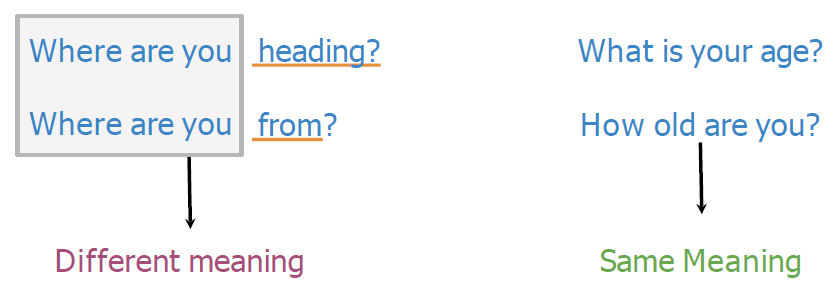
\includegraphics[width=\textwidth,height=0.8\textheight,keepaspectratio]{images/vector-space/why-vector-space.png}
    \end{figure}
    \begin{itemize}
        \item Words and sentences can have different meanings depending on context.
        \item Vector space models help capture semantic similarity and differences.
        \item Useful for tasks like paraphrase detection, question answering, and information retrieval.
    \end{itemize}
\end{frame}

\begin{frame}{Fundamental}
    \begin{figure}
        \centering
        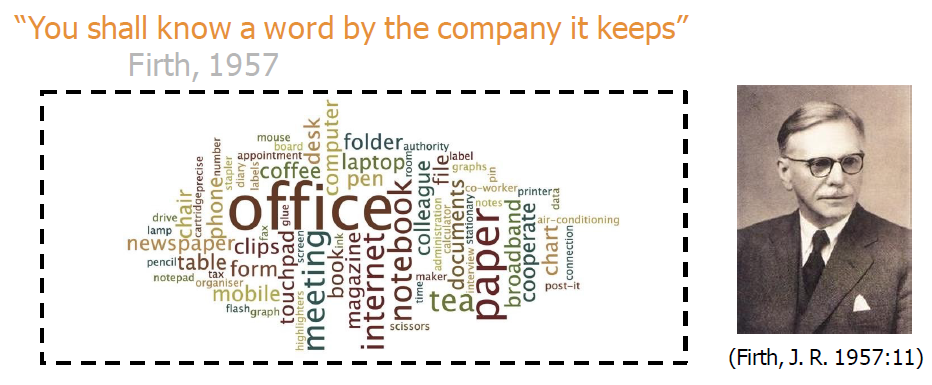
\includegraphics[width=\textwidth,height=0.8\textheight,keepaspectratio]{images/vector-space/vector-space-funda.png}
    \end{figure}
\end{frame}

\begin{frame}{Vector Space Models (VSM)}
    \begin{itemize}
        \item VSM represents words or documents as vectors in an $n$-dimensional space.
        \item Based on the \textbf{distributional hypothesis}: Words that occur in similar contexts have similar meanings.
        \item Forms the foundation for information retrieval, document classification, and word embeddings.
    \end{itemize}
\end{frame}

\begin{frame}{Vector Space Models – Formal Definition}
    \begin{itemize}
        \item A \textbf{term-document matrix}: Rows represent words (terms), columns represent documents (or vice versa).
        \item Each cell contains a value such as:
        \begin{itemize}
            \item Term Frequency (TF)
            \item TF-IDF (Term Frequency-Inverse Document Frequency)
            \item Co-occurrence count
        \end{itemize}
        \item The matrix is typically high-dimensional and sparse:
        \begin{itemize}
            \item Size = $|\text{Vocabulary}| \times |\text{Documents}|$
        \end{itemize}
    \end{itemize}
\end{frame}

\begin{frame}{Vector Space Model Applications}
    \begin{itemize}
        \item You eat \textit{cereal} from a \textit{bowl} $\rightarrow$ Capturing semantic similarity (paraphrase understanding)
        \item You \textit{buy} something and someone else \textit{sells} it $\rightarrow$ Capturing relational meaning (analogies)
    \end{itemize}
    \begin{figure}    \centering
        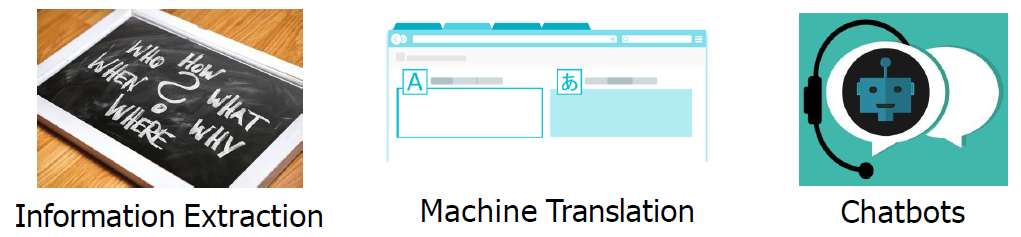
\includegraphics[width=\textwidth,height=0.8\textheight,keepaspectratio]{images/vector-space/vector-space-application.png}
    \end{figure}
\end{frame}

